\documentclass{exam}
\usepackage{mainExam}

\title{Produit Scalaire}
\author{Première Spécialité Mathématiques}
\date{4 Septembre 2024}

\begin{document}
\maketitle
\begin{questions}
\question Soit $\vect{u}$ et $\vect{v}$ tels que $\norm{\vect{u}} = 2$, $\norm{\vect{v}} = 3$ et $\widehat{\vect{u},\vect{v}} = 60°$. Calculer le produit scalaire $\vect{u} \cdot \vect{v}$.
\vspace*{0.5cm}

\question Soit $\vect{p}$ et $\vect{q}$ tels que $\norm{\vect{p}} = 5$, $\norm{\vect{q}} = \sqrt{3}$ et $\widehat{\vect{p},\vect{q}} = 135°$. Calculer le produit scalaire $\vect{p} \cdot \vect{q}$.
\vspace*{0.5cm}

\question Soit deux vecteurs $\vect{y}$ et $\vect{z}$ tels que $\norm{\vect{y}} = 6$, $\norm{\vect{z}} = 2$ et $\vect{y} \cdot \vect{z} = -2$. Déterminer une mesure de l'angle $\widehat{\vect{y};\vect{z}}$.
\vspace*{0.5cm}

\question Soit $ABC$ un triangle équilatéral de côté $5$. Calculer le produit scalaire $\vect{AB} \cdot \vect{AC}$.
\vspace*{0.5cm}

\question Soit $ABCD$ un carré de côté $5$. Calculer le produit scalaire $\vect{AB} \cdot \vect{AC}$.
\vspace*{0.5cm}

\question Soit $ABCD$ un carré de côté $4$ et de centre $O$. On place les points les milieux $I$, $J$, $K$ et $L$ respectifs des segments $[AB]$, $[BC]$, $[CD]$ et $[DA]$. Calculer les produits scalaires suivants:
\begin{parts}
\part $\vect{CO} \cdot \vect{CK}$
\part $\vect{CJ} \cdot \vect{LJ}$
\part $\vect{IJ} \cdot \vect{KL}$
\part $\vect{IJ} \cdot \vect{IL}$
\end{parts}
\vspace*{0.5cm}

\question Soit $ABCD$ un rectangle de centre $E$. On pose $F$ le symétrique de $E$ par rapport à la droite $(AB)$.
\begin{center}
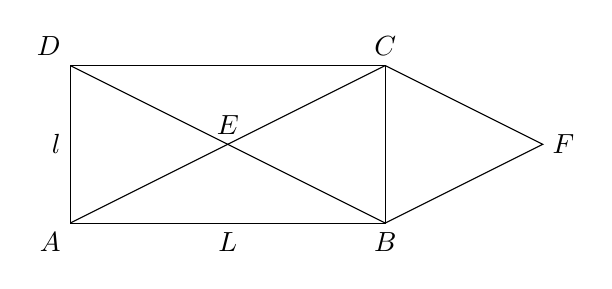
\begin{tikzpicture}
\coordinate (A) at (0,0);
\coordinate (B) at (4,0);
\coordinate (C) at (4,2);
\coordinate (D) at (0,2);
\coordinate (E) at (2,1);
\coordinate (F) at (6,1);

\draw (A) -- (B) node[midway,below] {$L$} -- (C) -- (D) -- cycle node[midway, left] {$l$};
\draw (A) -- (C);
\draw (B) -- (D);
\draw (B) -- (F) -- (C);
\draw (A) node[below left] {$A$};
\draw (B) node[below] {$B$};
\draw (C) node[above] {$C$};
\draw (D) node[above left] {$D$};
\draw (E) node[above] {$E$};
\draw (F) node[right] {$F$};
\end{tikzpicture}
\end{center}
Calculer les produits scalaires suivants en fonction de $L$ et de $l$ :
\begin{parts}
\part $\vect{BA} \cdot \vect{BE}$
\part $\vect{CF} \cdot \vect{CD}$
\part $\vect{AF} \cdot \vect{AB}$
\part $\vect{AB} \cdot \vect{BE}$
\part $\vect{BF} \cdot \vect{DC}$
\end{parts}

\newpage

\question Calculer à l'aide des indications suivantes le produit scalaire $\vect{AN} \cdot \vect{AM}$.
\begin{center}
\begin{tikzpicture}
\coordinate (A) at (0,0);
\coordinate (N) at (0,3);
\coordinate (B) at (6,0);
\coordinate (M) at (6,4);

\draw (A) node[below] {$A$} -- (N) node[midway,left] {$3$} node[above] {$N$};
\draw (A) -- (B) node[midway, below] {$6$} node[right] {$B$};
\draw (B) -- (M) node[midway,right] {$4$} node[above] {$M$};
\draw (A) -- (M);
\draw (B) -- (N);
\draw[thin] (A) ++(0,0.25) -- ++(0.25,0) -- ++(0,-0.25);
\draw[thin] (B) ++(0,0.25) -- ++(-0.25,0) -- ++(0,-0.25);
\end{tikzpicture}
\end{center} 
\end{questions}
\end{document}